\documentclass[9pt,twocolumn,twoside]{pnas-new}
\usepackage{textcomp}
\usepackage{caption}
\usepackage{subcaption}
\usepackage{siunitx}
\usepackage{multirow}
\usepackage{xr}
\usepackage[switch,columnwise]{lineno}
\usepackage[export]{adjustbox}

\usepackage{xcolor}
\newcommand{\todo}[1]{\textcolor{olive}{#1}}
\newcommand{\bwn}[2]{#1\textsuperscript{#2}}

\templatetype{pnasresearcharticle}

\title{Structural Basis for Ligand Modulation of the CCR2 Conformational Landscape}

% Use letters for affiliations, numbers to show equal authorship (if applicable) and to indicate the corresponding author
\author[a,b]{Bryn C. Taylor}
\author[a]{Christopher T. Lee}
\author[a,1]{Rommie E. Amaro}


\affil[a]{Department of Chemistry and Biochemistry, University of California San Diego, 9500 Gilman Drive, La Jolla, California, 92093}
\affil[b]{Biomedical Sciences Graduate Program, University of California San Diego}

\leadauthor{Taylor}

\significancestatement{CCR2 is an important immune system protein that is implicated in many immune and inflammatory diseases, including cancer. Numerous clinical and pre-clinical trials are attempting to target CCR2 to find an effective therapy. To support drug discovery efforts, we use atomic simulations and Markov-state models to investigate the conformational landscape of CCR2; information that is unattainable by experimental methods.}

\authorcontributions{B.C.T, C.T.L, and R.E.A. designed research; B.C.T. performed the research; B.C.T. and C.T.L. analyzed the results; and B.C.T., C.T.L, and R.E.A. wrote the paper.}
\authordeclaration{The authors declare the following competing financial interest(s): REA has equity interest in, and is a cofounder and scientific advisor of, Actavalon, Inc.}
\correspondingauthor{\textsuperscript{1}To whom correspondence should be addressed. E-mail: ramaro$@$ucsd.edu}

\keywords{CC Chemokine Receptor 2 $|$ CCR2 $|$ GPCR $|$ Markov State Models}

% Abstract
\begin{abstract}
CC Chemokine Receptor 2 (CCR2) is a part of the chemokine receptor family, an important class of therapeutic targets.
These class A G-protein coupled receptors (GPCRs) are involved in mammalian signaling pathways and control cell migration toward endogenous CC chemokine ligands, named for the adjacent cysteine motif on their N-terminus.
Chemokine receptors and their associated ligands are involved in a wide range of diseases and thus have become important drug targets.
CCR2, in particular, promotes the metastasis of cancer cells and is also implicated in autoimmunity driven type-1 diabetes, diabetic nephropathy, multiple sclerosis, asthma, atherosclerosis, neuropathic pain, and rheumatoid arthritis.
Although promising, CCR2 antagonists have been largely unsuccessful to date.
Here, we investigate the effect of an orthosteric and an allosteric antagonist on CCR2 dynamics by coupling long timescale molecular dynamics simulations with Markov-state model theory.
We find that the antagonists shift CCR2 into several stable inactive conformations that are distinct from the crystal structure conformation and disrupt a continuous internal water and sodium ion pathway, preventing transitions to an active-like state.
Several metastable conformations present a cryptic drug binding pocket near the allosteric site that may be amenable to targeting with small molecules.
Without antagonists, the apo dynamics reveal intermediate conformations along the activation pathway that provide insight into the basal dynamics of CCR2, and may also be useful for future drug design.
\end{abstract}



\dates{This manuscript was compiled on \today}
%\doi{\url{www.pnas.org/cgi/doi/10.1073/pnas.XXXXXXXXXX}} %just for PNAS

\begin{document}
%\linenumbers
\verticaladjustment{-2pt}

\maketitle
\thispagestyle{firststyle}
\ifthenelse{\boolean{shortarticle}}{\ifthenelse{\boolean{singlecolumn}}{\abscontentformatted}{\abscontent}}{}

%\subsection*{Submitting Manuscripts}
%All authors must submit their articles at \href{http://www.pnascentral.org/cgi-bin/main.plex}{PNAScentral}. If you are using Overleaf to write your article, you can use the ``Submit to PNAS'' option in the top bar of the editor window.


% Introduction...
The signaling axis of CCR2 and its endogenous ligand, CCL2, is a notable therapeutic target due to its association with numerous diseases, including cancer, autoimmunity driven type-1 diabetes, diabetic nephropathy, multiple sclerosis, asthma, atherosclerosis, neuropathic pain, and rheumatoid arthritis\cite{Ben-Baruch2006,OConnor2015,Solomon2010}.
Despite much effort that has been devoted to clinical and pre-clinical trials, a successful antagonist has yet to be developed\cite{Pease2009, Pease2009a, Scholten2012,Lim2016,Solari2015,Horuk2009,https://www.clinicaltrials.gov} (http://www.clinicaltrials.gov).
Prior to a full-length crystal structure of CCR2, several studies used homology modeling and docking to gain insights into the structure and dynamics of the protein and its associated ligands or small molecule drugs\cite{Shahlaei2013,Chavan2012,Kothandan2012}.
However, recently CCR2 was crystallized for the first time\cite{Zheng2016}, opening up new opportunities for rational drug design.

\begin{SCfigure*}[\sidecaptionrelwidth][h]
\centering
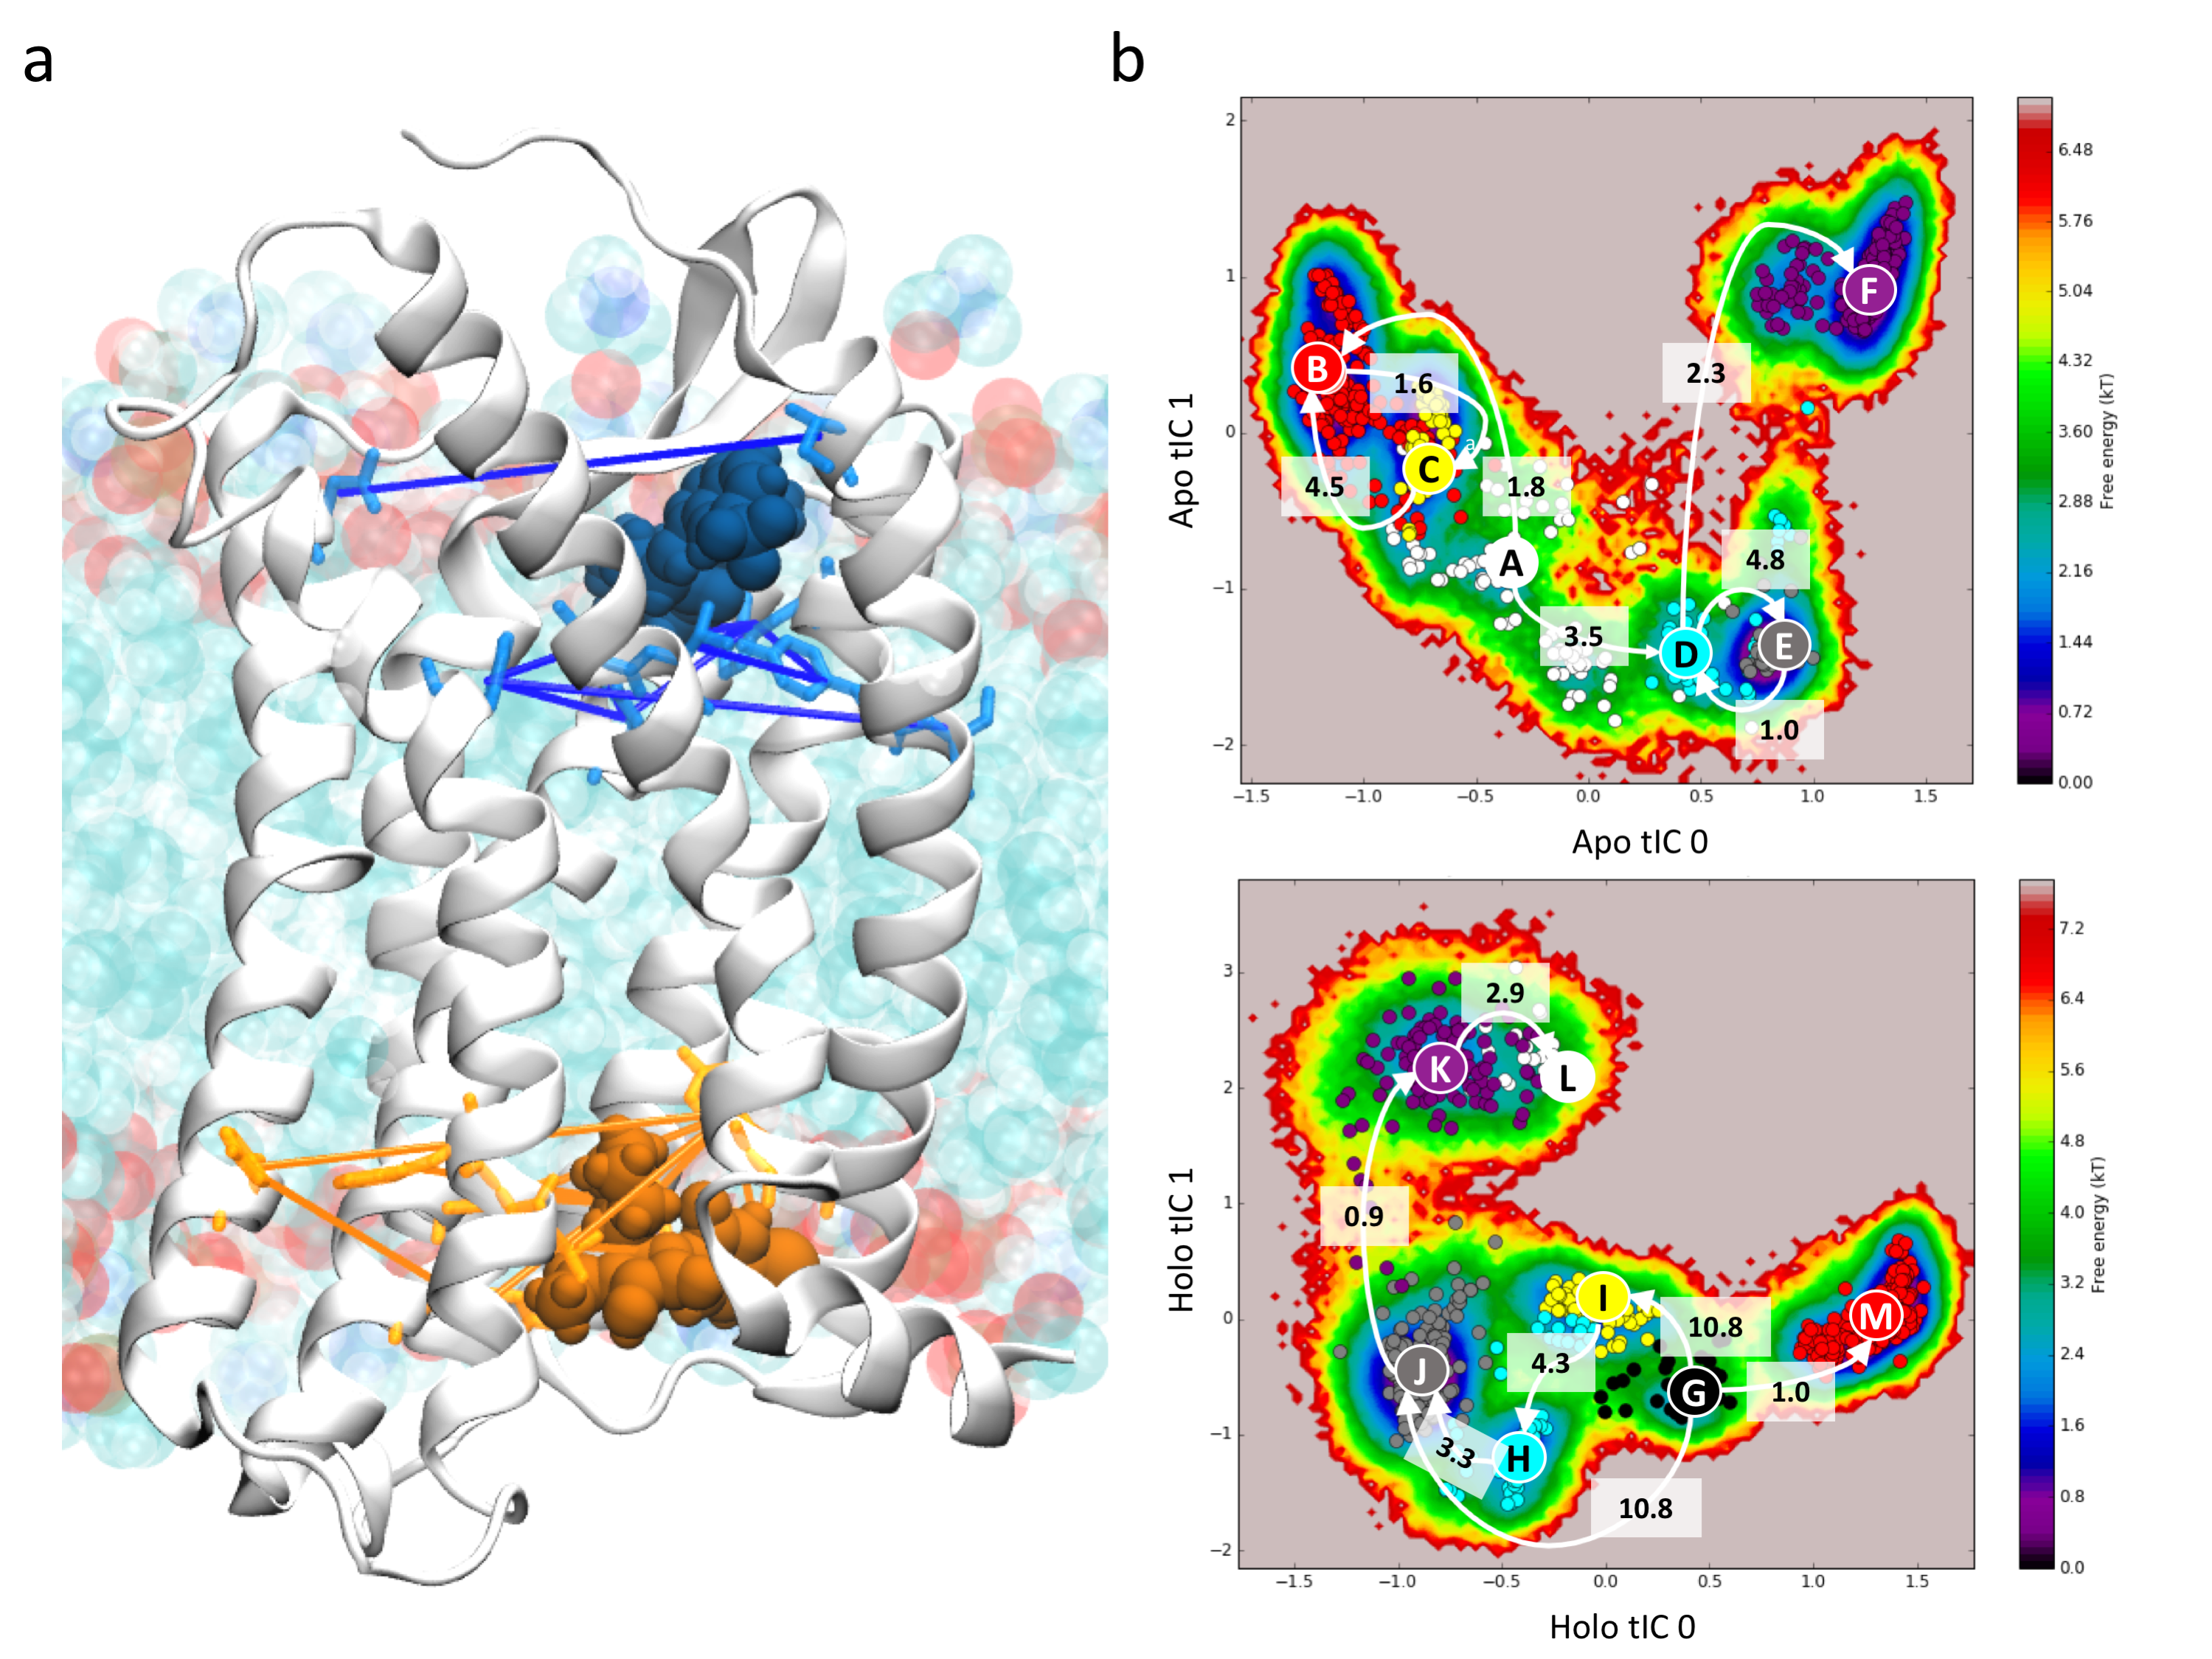
\includegraphics[width=11.4cm]{apo_holo_hmm.eps}
\caption{MD simulations of CCR2 in a lipid bilayer were performed apo and holo CCR2. A) Sets of residue pairs surrounding the two ligand binding pockets were used with TICA (SI Appendix). The protein is shown in white cartoon. Lipids are teal, red, and blue. The orthosteric and allosteric ligands are shown in blue and orange, respectively, with inter-residue pair distances denoted by similarly colored lines. The free energy and Maximum-Likelihood HMMs of B) apo and C) holo CCR2, projected onto the first two TICA components. Coarse-grained states are labeled and colored. Transition rates between macrostates are represented by arrows reported in units of ms$^{-1}$.}
\label{fig:apo_holo_hmm}
\end{SCfigure*}

As with most GPCRs, chemokine receptors transmit signals across cell membranes by means of extracellular ligand and intracellular G-protein binding.
Distinct conformational states of the receptor are necessary for chemokine/ligand binding, G-protein binding, activation, inactivation, and signal transmission \cite{Latorraca2017, Venkatakrishnan2013, Zhang2018}.
GPCRs are no longer considered to be simple on/off molecular switches -- instead, they assume a wide range of conformational states, including ligand-specific states, intermediate states, and states that allow for basal (apo) signaling without ligands bound \cite{Venkatakrishnan2013, Katritch2013, Manglik2015, Katritch2012, Malik2013, Yao2009, Nygaard2013, Bockenhauer2011}.
Ligands and small molecule drugs may shift the equilibrium of the receptor's conformational states towards particular states.
Effective small molecule antagonists that inhibit CCR2 signaling, potentially by shifting the receptor equilibrium toward inactive conformational states, are desired for treatment of diseases that involve the CCR2/CCL2 axis.
Key challenges are to characterize the basal dynamics of CCR2 and to understand how current antagonistic small molecule drugs modulate these dynamics.
While crystal structures provide valuable snapshots of proteins and protein complexes, they lack the ability to reveal dynamics at the atomic level.
Starting with the newly resolved crystal structure of CCR2 (PDB ID: 5T1A) we performed multi-microsecond all-atom explicitly solvated molecular dynamics (MD) simulations of the receptor in a lipid bilayer in unbound (apo) and dual-antagonist-bound (holo) states (Fig. \ref{fig:apo_holo_hmm}).
The two antagonists were co-crystallized with CCR2: the orthosteric antagonist, BMS-681, and the allosteric antagonist, CCR2-RA-[R].
Each system was simulated in triplicate on Anton 2 \cite{Shaw2014} for a total of 260 microseconds (SI Appendix, Table S1, Fig. S1).

While long timescale (tens of microseconds) simulations are useful for analyzing sequential conformational changes, simulations are generally unable to directly probe timescales of biological interest (milliseconds - seconds)\cite{Bowman2011}.
One way to bridge this timescale gap is to couple MD simulations with Markov state model theory\cite{Swope2004, Singhal2004, Malmstrom2014, Amaro2018, Amaro2018a, Bowman2014, Noe2007, Prinz2011a, Schutte1999} (MSM, described in SI Materials and Methods).
Integrating  MD simulations with MSMs allowed us to extend the reach of simulated timescales, and identify key differences in the conformational ensembles and dominant slow motions of apo and holo CCR2.
We find that the antagonists disrupt a continuous internal water and sodium ion pathway preventing transitions to an active-like state, and shift CCR2 into several stable states that are distinct from the crystal structure conformation, three of which present a cryptic druggable pocket.
Without antagonists, intermediate conformations with active-state conformational signatures shed light on the apo dynamics of CCR2 and may also be useful for future drug design.

%%%% 2a_results
\section*{Results and Discussion}

To compare the conformational landscapes of apo and holo CCR2 we ran all-atom MD simulations totalling 260 $\mu$s on Anton 2\cite{Shaw2014}.
For one MD replicate of the holo system, we observed the orthosteric drug dissociate from the protein.
Analyzing the conformations before and after ligand dissociation yields a first glimpse of the allosteric effect of the remaining antagonist on the protein dynamics, and provides a starting point for future rounds of adaptive sampling to obtain robust dissociation statistics (not pursued here).
In order to extend the analysis beyond a dissociation event and connect to longer timescale phenomena, MSMs were constructed from the trajectories.
The variational approach for conformation dynamics\cite{Noe2013}, specifically Time-structure-based independent component analysis (TICA)\cite{Schwantes2013, Perez-Hernandez2013} was used to perform dimensionality reduction for the MSMs and identify the features and collective variables (time-structure based independent components (TICs)) that best represent the dominant slow motions.
The MSMs create human interpretable models that we use to interrogate the conformational and kinetic differences between the two ensembles to derive new understandings about the mechanisms underlying effects of CCR2 antagonism. 
Further methodological details are provided in Methods and in the SI Appendix. 

%%%% 2b_results
\subsection*{Comparison of the CCR2 conformational ensemble with other class A GPCRs}

We compare representative states from the apo and holo conformational ensemble with other class A GPCRs to establish similarities within the class.
We find that the states of apo CCR2 have conformational signatures found in the active or intermediately-active states of GPCRs, suggesting that these states are on a pathway toward activation.
Holo CCR2 diverges from the crystal structure to form distinct states that expose putative drug binding pockets and reveal the effect of antagonists on receptor dynamics.

We evaluate the metastable states by comparing helical conformational signatures and conserved groups of structurally neighboring amino acids called 'microswitches'.
These include NPxxY (\bwn{Tyr 305}{7.53}), DRY (\bwn{Arg 138}{3.50}), \bwn{Tyr 222}{5.58}, sets of residues in the orthesteric and allosteric binding sites, and the chemokine and G-protein binding pockets to the inactive crystal structure of CCR2 that we used in this study (PDB ID: 5T1A), to an intermediately-active crystal structure of a class A GPCR, A\textsubscript{2A}AR(PDB ID: 2YDO\cite{Lebon2011}; 25\% sequence identity to CCR2), the active crystal structure of a class A GPCR, US28 (PDB ID: 4XT3\cite{Burg2015}; 30\% sequence identity to CCR2), and three other chemokine receptors: CCR5 (PDB ID: 4MBS\cite{Tan2013}, CCR9 (PDB ID: 5LWE\cite{Oswald2016}), and CXCR4 (PDB ID: 4RWS\cite{Qin2015}).
Signatures of an active GPCR state include:
1) the inward shift of the intracellular part of helix VII toward the helical bundle,
2) the outward shift of the intracellular part of helix VI in concert with helix V,
3) the upward shift and lateral movement of helix III,
and 4) the rearrangements of conserved microswitches \cite{Katritch2013}.
According to these metrics, the starting crystal structure of CCR2 is in an inactive conformation\cite{Zheng2016}, the crystal structure of A\textsubscript{2A}AR is an an intermediately-active conformation, and the crystal structure of US28 is in the active conformation.

\begin{SCfigure*}[\sidecaptionrelwidth][h]
\centering
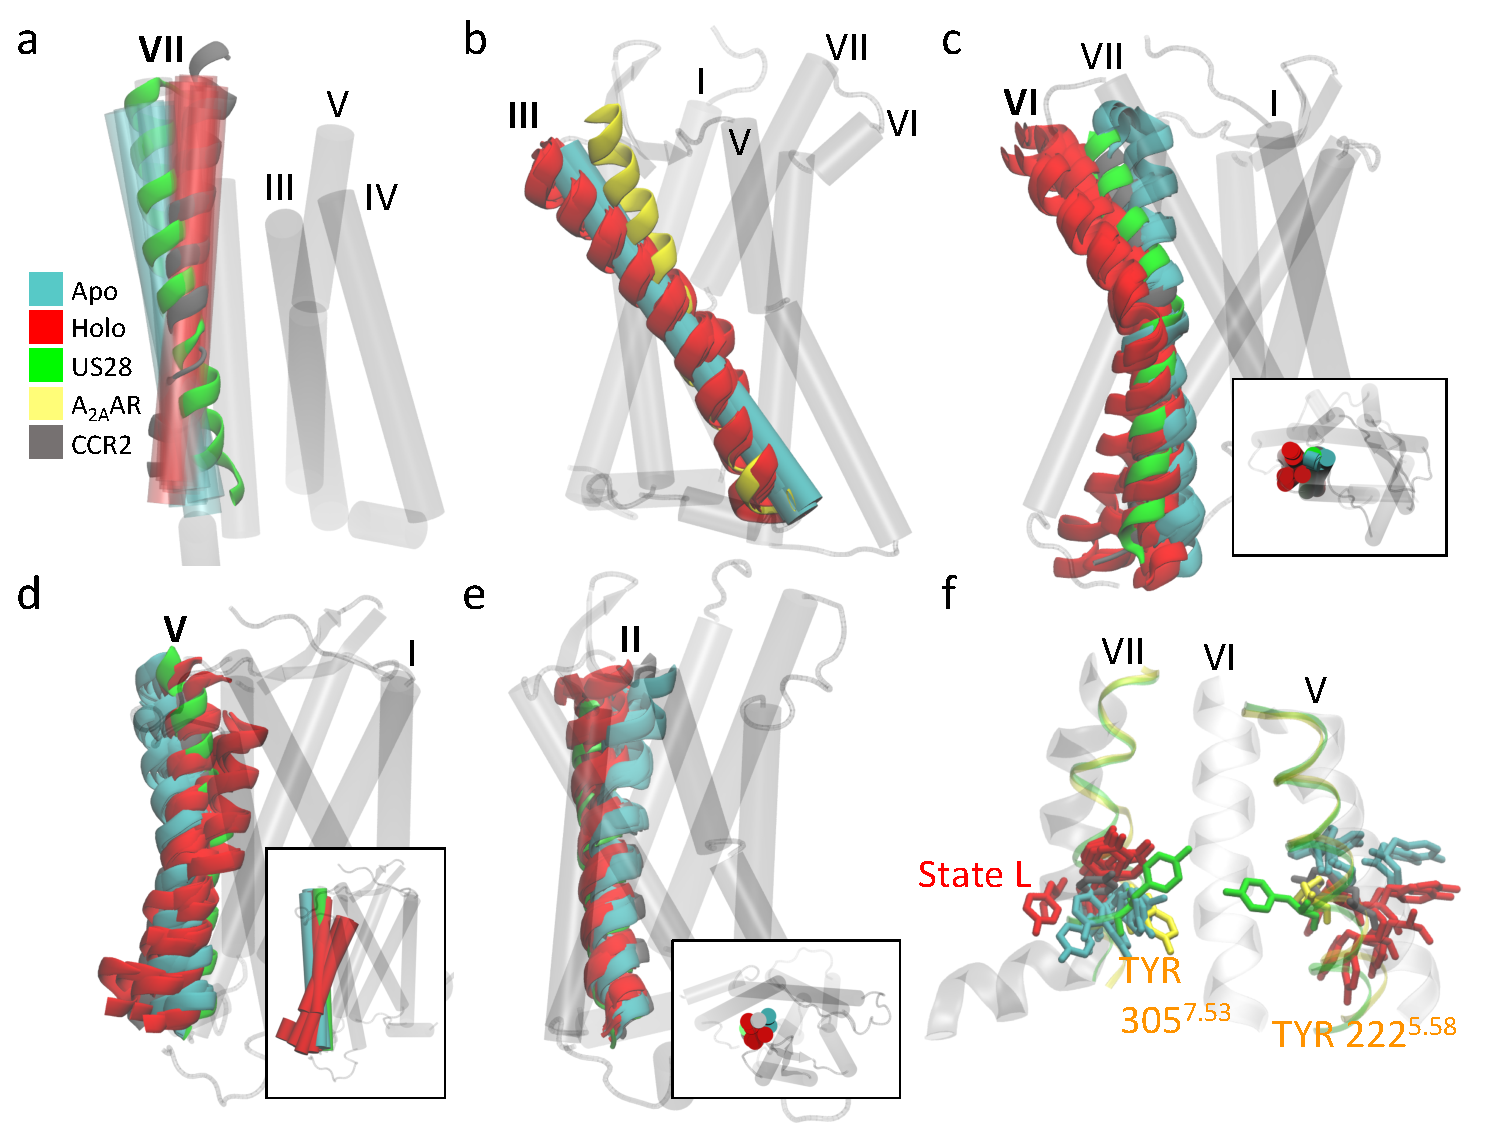
\includegraphics[width=11.4cm]{global_tm.pdf}
\caption{Apo and holo macrostates are compared to the active crystal structure of US28 (green, PDB ID 4XT3) or the active crystal structure of A\textsubscript{2A}AR (yellow, PDB ID 2YDO) and the crystal structure of CCR2 (grey, PDB ID 5T1A). A) Helix VII of apo macrostates resemble the active conformation of US28; holo macrostates resemble the CCR2 crystal structure. B) The conformation of helix III in apo macrostates subtly resemble active A\textsubscript{2A}AR; holo macrostates are tilted away from the center of the helical bundle. C,D) Helix V and VI of apo macrostates straighten or tilt in toward the center of the protein, similar to the active conformation of US28 and the inactive CCR2 crystal structure; helix V and VI of several holo macrostates tilt away from the binding sites, accessing more active-like conformations than the apo macrostates or even the active state of US28. E) Helix II in the apo macrostates shifts inward; in the holo macrostates it shifts outward. F) In licorice are conserved motifs TYR 305\textsuperscript{7.53} and TYR 222\textsuperscript{5.58}. All six apo metastable state assume a new conformation for TYR 305\textsuperscript{7.53}, pointing intracellulary and in a similar conformation to active A\textsubscript{2A}AR. Six out of the seven holo metastable states have TYR 305\textsuperscript{7.53} in the same conformation as the equilibrated crystal structure. Post-ligand-dissociation holo state L assumes a new position of TYR 305\textsuperscript{7.53}, more similar to the dominant apo conformation. Apo metastable states sample a narrower range of conformations for TYR 222\textsuperscript{5.58} than holo.}
\label{fig:global_tm}
\end{SCfigure*}

\subsubsection*{1) Apo macrostates show an active-like inward shift of the intracellular part of helix VII toward the helical bundle}
All of the apo macrostates exhibit an active state hallmark (Fig. \ref{fig:global_tm}A): the intracellular end of helix VII tilts slightly inward toward the center of the helical bundle.
More prominently, the extracellular end of helix VII tilts outward, resembling the active conformation of US28.
The holo macrostates show the opposite: the intracellular end of helix VII tilts slightly outward and the extracellular end of helix VII tilts inward, remaining in the crystal structure conformation.

\subsubsection*{2) Holo macrostates, not apo, show an active-like outward shift of the intracellular part of helix VI in concert with helix V}
Helix V and VI in the apo macrostates are not in an active conformation.
Instead, it is the holo macrostates that have the intracellular end of helix V and VI tilting outward to resemble the active conformation (Fig. \ref{fig:global_tm}C,D), suggesting that neither apo nor holo macrostates are in an exclusively inactive or active conformational state, despite starting from a particularly inactive crystal structure.
Due to this outward motion of helix VI, holo macrostates K and L exhibit a more open G-protein binding site compared to holo macrostate G which is more closed. The RMSF of the allosteric ligand is larger in macrostates K and L, indicating that the inactive (inward) conformation of helix VI may play a critical role in stabilization of the allosteric ligand (SI Appendix, Fig. S2).

\subsubsection*{3) Apo macrostates show an active-like upward shift and lateral movement of helix III}
Apo macrostates also resemble the active conformation by the slight upward shift of helix III; unlike holo macrostates, which remain in a position similar to the inactive crystal structure (Fig. \ref{fig:global_tm}B).

\subsubsection*{4) The rearrangements of conserved microswitches suggest that apo macrostates are active intermediates, and holo macrostates are inactive intermediates}
\emph{a) NPxxY motif (Tyr 305\textsuperscript{7.53}).}
In the inactive conformation of GPCRs, Tyr 305\textsuperscript{7.53} points towards helices I, II, or VIII (in CCR2, it points toward II), and in the active state Tyr 305\textsuperscript{7.53} points toward middle axis of helical bundle\cite{Katritch2013}.
Each apo macrostate shows Tyr 305\textsuperscript{7.53} pointing downward into the intracellular (G-protein) binding pocket (Fig. \ref{fig:global_tm}F).
This positioning of Tyr 305\textsuperscript{7.53} matches the intermediately-active conformation of A\textsubscript{2A}AR, which also points down. It does not match the active conformation in US28 that points up, and is also distinct from the inactive crystal structure of CCR2.
In six out of the seven the holo macrostates, Tyr 305\textsuperscript{7.53} is stabilized in the inactive state and matches the inactive CCR2 crystal structure conformation as well as the inactive chemokine receptor crystal structures of CCR5 and CCR9.

The holo macrostate in which Tyr 305\textsuperscript{7.53} is not stabilized in the inactive conformation is accessed after the orthosteric ligand dissociates (State L, Fig. \ref{fig:apo_holo_hmm}C, \ref{fig:global_tm}F); the allosteric pocket residues rearrange and Tyr 305\textsuperscript{7.53} assumes a downward conformation similar to the apo states and the crystal structure of CXCR4.
These concerted events may indicate allosteric cross-talk between the chemokine binding site and the G-protein binding site.

\emph{b) The microswitch residue Trp 256\textsuperscript{6.48}, and the interaction of the DRY motif (Arg 138\textsuperscript{3.50}) with Tyr 222\textsuperscript{5.58}.}
Apo and holo macrostates both maintain the same chi angle of the conserved microswitch residue Trp 256\textsuperscript{6.48} which describes an active GPCR when it switches from gauche to trans conformation and facilitates the interaction of Tyr 222\textsuperscript{5.58} and Tyr 305\textsuperscript{7.53}.
In the CCR2 crystal structure and the crystal structures of chemokine receptors CCR5 and CXCR4, Trp 256\textsuperscript{6.48} points upward and extends into the helical core.
Each apo macrostate shows Trp 256\textsuperscript{6.48} in a single conformation pointing toward helix III (SI Appendix, Fig. S3).
In the holo macrostates, Trp 256\textsuperscript{6.48} access three distinct conformations: one resembling the crystal structure but with the helix shifted slightly outward from the helical core, another that laterally twists toward helix V, and one conformation that points down into the helical core toward the G-protein binding site (SI Appendix, Fig. S3).
This third conformation, in which the orthosteric ligand has dissociated, represented by the holo macrostate L, further suggests cross-talk between the chemokine binding site and the rest of the protein.

The interaction of these two tyrosines and Arg 138\textsuperscript{3.50} also characterizes an active state GPCR \cite{Caliman2015}.
In the inactive crystal structure of CCR2, Tyr 222\textsuperscript{5.58} points toward lipids, sterically blocked by Phe 246\textsuperscript{6.38} from interaction with Arg 138\textsuperscript{3.50} and Tyr 305\textsuperscript{7.53} \cite{Zheng2016}.
In apo macrostates, Tyr 222\textsuperscript{5.58} remains pointed toward the lipids, never swiveling around to interact with Arg 138\textsuperscript{3.50} or Tyr 305\textsuperscript{7.53} as occurs in activated GPCR states (Fig. \ref{fig:global_tm}F).
Holo macrostates actually show increased range of motion of Tyr 222\textsuperscript{5.58}, diverging from the crystal structure and stabilizing in unique intermediate conformations.
The steric obstruction from Phe 246\textsuperscript{6.38} is alleviated in both apo and holo macrostates, as Phe 246\textsuperscript{6.38} swings outward and points toward the lipids.
The conformations of these microswitch residues indicate that both apo and holo macrostates are sampling different conformations.


\subsubsection*{\textbf{5) Formation of continuous water pathway suggests movement of apo towards activation}}
Internal water molecules, which may influence conformational changes in GPCRs by interfering with hydrogen bonding networks of the receptor's backbone and side chains, are postulated to be an integral part of receptor activation in GPCRs\cite{Jastrzebska2011, Angel2009,Choe2011, Huang2015}.
Work in other GPCRs has additionally shown that activation can allow water and sodium ion flow through GPCR core\cite{Yuan2014}.
Furthermore, it has been shown that the activation of GPCRs is voltage sensitive\cite{Rinne2013}.
Our simulations enable the direct visualization of water and sodium ion density in both CCR2 ensembles.

A continuous internal water pathway forms in apo CCR2 (Fig. \ref{fig:water_na}A).
The antagonists disrupt this water pathway, slowing the rate of water entry to and egress from the protein core (Fig. \ref{fig:water_na}A).
An analysis of the water occupancy per residue (SI Appendix, Fig. S4A) indicates that several of the high water occupancy residues (e.g. Asp 36\textsuperscript{1.26}, Ser 50\textsuperscript{1.40}, Glu 235\textsuperscript{6.27}, Lys 236\textsuperscript{6.28}, Glu 310\textsuperscript{8.48}, Lys 311\textsuperscript{8.49}) may be exposed to more water in the apo simulations than in the holo simulations simply because the ligands have been removed and the water has access to the binding pockets.
The other residues (e.g., Asp 78\textsuperscript{2.40}, Tyr 80\textsuperscript{2.42}, Asp 88\textsuperscript{2.50}, Leu 92\textsuperscript{2.54}, Ile 93\textsuperscript{2.55}, Gly 127\textsuperscript{3.39}, Ile 128\textsuperscript{3.40}, Glu 291\textsuperscript{7.39}, and Phe 312\textsuperscript{8.50}) reside in the protein core, along the continuous pathway (Fig. \ref{fig:water_na}A).

Class A GPCRs also possess a conserved sodium binding site at \bwn{Asp}{2.50} corresponding to Asp 88 in CCR2\cite{Katritch2014}.
The dynamics of activation was previously hypothesized to impinge upon the sodium binding pocket, eventually leading to ion permeation into the cytosol\cite{Vickery2018}.
A sodium ion occupancy per residue analysis (SI Appendix, Fig. S4B) indicates that, while no sodium permeation events were observed in the apo trajectories, ions interact with residues \bwn{Asp 88}{2.50}, \bwn{Glu 291}{7.39}, and \bwn{His 297}{7.45} which form and surround the sodium binding site.
In holo CCR2, the ligands do not permit sodium ions to enter the protein core; instead, ions interact primarily with residues Glu 270\textsuperscript{6.62} and His 317\textsuperscript{8.55}-Lys 320\textsuperscript{8.58}.

\begin{figure}[h]
\centering
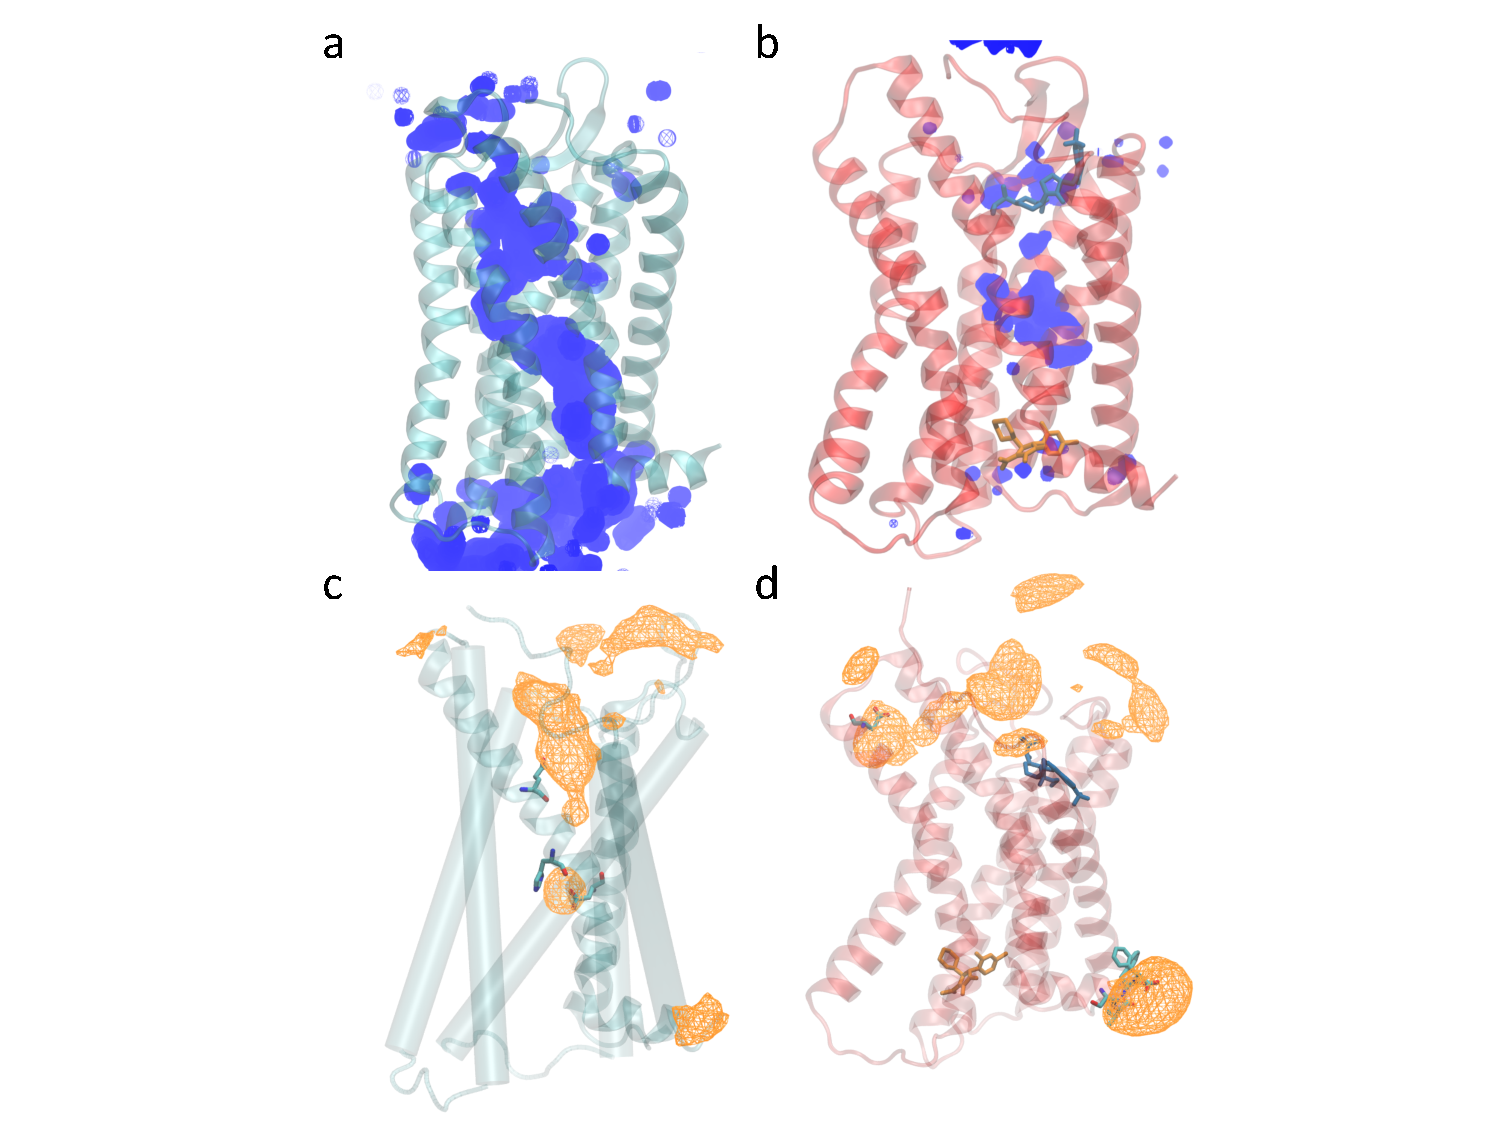
\includegraphics[width=8.7cm]{water_na_internal.pdf}
\caption{Ligands disrupt a continuous internal water and sodium ion pathway. Average water density over a 50 microsecond simulation of A) apo (teal) and B) holo (red). The orthosteric ligand is shown in blue and the allosteric ligand is shown in orange. Total average sodium ion density in C) apo and D) holo. Highest occupancy residues are depicted in cyan licorice and plotted in SI Appendix Fig. S4.}
\label{fig:water_na}
\end{figure}

%%%% 2c_results
\section*{Effects of antagonist binding on CCR2 dynamics}

Comparisons of the apo and holo MSMs elucidate the effects of antagonists on CCR2 dynamics.
Notably, apo relaxation timescales are an order of magnitude less than holo relaxation timescales (SI Appendix, Table S2), indicating that the antagonists greatly perturb CCR2 dynamics.
The motions described by apo and holo TIC 0 represent the most striking difference between the two systems' dynamics.
In the apo MSM, the inter-residue distances most closely correlated with apo TIC 0 are all a part of the allosteric (G-protein) binding pocket, whereas in the holo MSM, the inter-residue distances most closely correlated with holo TIC 0 are all a part of the orthosteric (chemokine) binding pocket (SI Appendix, Fig. S5).

Apo TIC 1 represents the flipping of Trp 98\textsuperscript{2.60} into the orthosteric drug binding site (Fig. S7A,B, SI Appendix, Fig. S5C).
In the crystal structure Trp 98\textsuperscript{2.60} packs with the tri-substituted cyclohexane of the orthosteric antagonist, BMS-681\cite{Zheng2016}.
Without the presence of this ligand, Trp 98\textsuperscript{2.60} assumes three distinct positions.
The Trp 98\textsuperscript{2.60} conformation in the cluster at the neutral TIC (boxed in yellow, Fig. S7A,B) most closely resembles the conformation of Trp 98\textsuperscript{2.60} in the active GPCR US28, which is shifted slightly up and in towards the helical core in comparison to the CCR2 crystal structure.
The two other conformations are found at the extreme ends of apo TIC 1 in densely populated free energy wells.
Of these two conformations, state F assumes the most dramatic conformation and protrudes into the chemokine binding site (SI Appendix, Fig. S6).
In the holo macrostates there is markedly less intrusion into the binding pocket due to the presence of the ligand.

Holo TIC 1 represents the concerted movement of 5 pairs of residues in the orthosteric ligand binding site during orthosteric ligand dissociation (Fig. S7C,D; SI Appendix, Fig. S5D).
The separation projected in the first two TICs (Fig. S7D) is divided into clusters of frames that occur before (white clusters), during (grey), and after (black) dissociation.
The residue pairs identified by TICA that contribute to holo TIC 1 and this ligand dissociation (SI Appendix, Fig. S5D) were confirmed by analyzing the original simulation data.
The key changes are the change in distance between Tyr 49\textsuperscript{1.39} - Thr 292\textsuperscript{7.40}, Trp 98\textsuperscript{2.60} - Tyr 120\textsuperscript{3.32}, Ser 50\textsuperscript{1.40} - Tyr 259\textsuperscript{6.51}, and the chi angle of Glu 291\textsuperscript{7.39}.
Notably, four of these residues (Tyr 49\textsuperscript{1.39}, Trp 98\textsuperscript{2.60}, Tyr 120\textsuperscript{3.32}, and Thr 292\textsuperscript{7.40}) are not only involved in binding to the co-crystallized orthosteric antagonist BMS-681 and/or CCL2 binding, but are also critical for GPCR activation \cite{Berkhout2003, Hall2009}.

The positioning of the orthosteric ligand and the conformation of Trp 98\textsuperscript{2.60} are closely linked (SI Appendix, Fig. S7C, Fig. S8).
After ligand dissociation, in holo states K and L (purple and white, respectively), Trp 98\textsuperscript{2.60} turns towards helix III, bending slightly inward toward the chemokine binding site.
Prior to ligand dissociation, Trp 98\textsuperscript{2.60} has two distinct conformations.
In the first conformation (states I and G, black and yellow), the ligand positions itself between helices I and VII, in the same conformation as the crystal structure.
Trp 98\textsuperscript{2.60} is constrained in a downward position, pointing intracellularly, also resembling the CCR2 crystal structure conformation and the crystal structure of chemokine receptor CCR5.
In the second conformation (States H and J, cyan and grey), Trp 98\textsuperscript{2.60} flips up and out of the binding pocket, pointing extracellularly, and the ligand moves between helices I and II. This conformation of Trp 98\textsuperscript{2.60} closely resembles the conformation of chemokine receptor CCR9.
The third conformation of Trp 98\textsuperscript{2.60} is found in State M (red), and is the most prominent position of the residue as it extends deeper into the chemokine binding site toward helix III.
In this case, the ligand interacts with helices II, IV, and V, and there are no transitions from this state to a dissociated state.

As in the apo MSM, the absence of the orthosteric ligand causes a shift in the position of Trp 98\textsuperscript{2.60}.
In the holo simulations shown in SI Appendix, Fig. S9, the dissociation event is preceded by a doubling of the distance between Trp 98\textsuperscript{2.60} and Tyr 120\textsuperscript{3.32}, and 3 $\mu$s after dissociation the distance returns to its previous 0.4 nm.
This increase in distance may be required for the ligand to begin the process of dissociating.
Another drastic change during the dissociation event is the switch of Glu 291\textsuperscript{7.39} from a constrained chi angle of -50 to -100 degrees to an unconstrained chi angle (SI Appendix, Fig. S10).
After dissociation, this angle more closely resembles the conformation in all apo simulations.

In the CCR2 crystal structure, there is a hydrogen bond between Tyr 49\textsuperscript{1.39} and Thr 292\textsuperscript{7.40}.
The gamma-lactam secondary exocyclic amine of the orthosteric ligand forms a hydrogen bond with the hydroxyl of Thr 292\textsuperscript{7.40}, and the carbonyl oxygen of the gamma-lactam forms a hydrogen bond with Tyr 49\textsuperscript{1.39}.
During simulation, the distance between Tyr 49\textsuperscript{1.39} and Thr 292\textsuperscript{7.40} remains stable until 3 $\mu$s after the ligand dissociates, when it begins fluctuating (SI Appendix, Fig. S11).
This suggests that the orthosteric ligand dissociation breaks the hydrogen bond between these key ligand binding residues.
This motion is captured in the holo MSM: the separation of the two residues is exemplified between States H (pre-dissociation) and L (post-dissociation) in SI Appendix, Fig. S11.

Finally, the faster dominant motions (TICs 2, 3, 4) in the holo MSM consist of rearrangements in the allosteric ligand binding site, suggesting that an allosteric rearrangement must first happen in order for the orthosteric ligand to dissociate.
Further evidence for this is the observed correlated motion of the downward flip of the conserved residue Tyr 305\textsuperscript{7.53} in the G-protein binding site with the dissociation of the orthosteric ligand from the chemokine binding site.

Overall, holo macrostates show more helical tilting and binding site expansion, which increases the solvent-accessible surface area (SASA) when compared to the crystal structure and the apo macrostates.
However, the apo simulations overall have greater residue fluctuation, suggesting that the antagonist ligands dampen CCR2 dynamics (SI Appendix, Fig. S12).

\subsection*{\textbf{Opening of a cryptic druggable pocket}}

A dramatic expansion of the extracellular (chemokine) binding site is exhibited in the holo macrostates.
The expansion is caused by a pronounced outward tilting of helix VI and slight outward tilting of helix II in the holo macrostates, whereas the apo macrostates show the opposite, with a slight inward tilting of both helices VI and II (Fig. \ref{fig:global_tm}C,E).
The intracellular (G-protein) binding site also enlarges in the holo macrostates due to the outward shift of the intracellular ends of helices V and VI, but remains obstructed in all apo and holo states.
In the crystal structure, this obstruction occurs by the interaction of Arg 138\textsuperscript{3.50} with Asp 137\textsuperscript{3.49} and with Thr 77\textsuperscript{2.39} \cite{Zheng2016}, which are maintained throughout all the simulations.
The outward movement of the intracellular end of helix VI and the movement of helix V toward helix VI in states L, J, and H in the holo MSM create a putative site for novel allosteric antagonists; this pocket also transiently appears in the apo simulations (Fig. \ref{fig:allo_pkt}).
Computational solvent mapping\cite{Kozakov2015} of this novel site indicates that the pocket presents surfaces that are amenable to ligand binding due to its ability to bind clusters of multiple different drug-like probes (Fig. \ref{fig:allo_pkt}C).
The pocket can be accessed through the lipid bilayer between helices IV and V, or from the G-protein binding site, as a deeper extension of the current allosteric binding site of CCR2-RA-[R], and may be useful for rational drug design or modification of current antagonists.

\begin{figure}[ht]
\centering
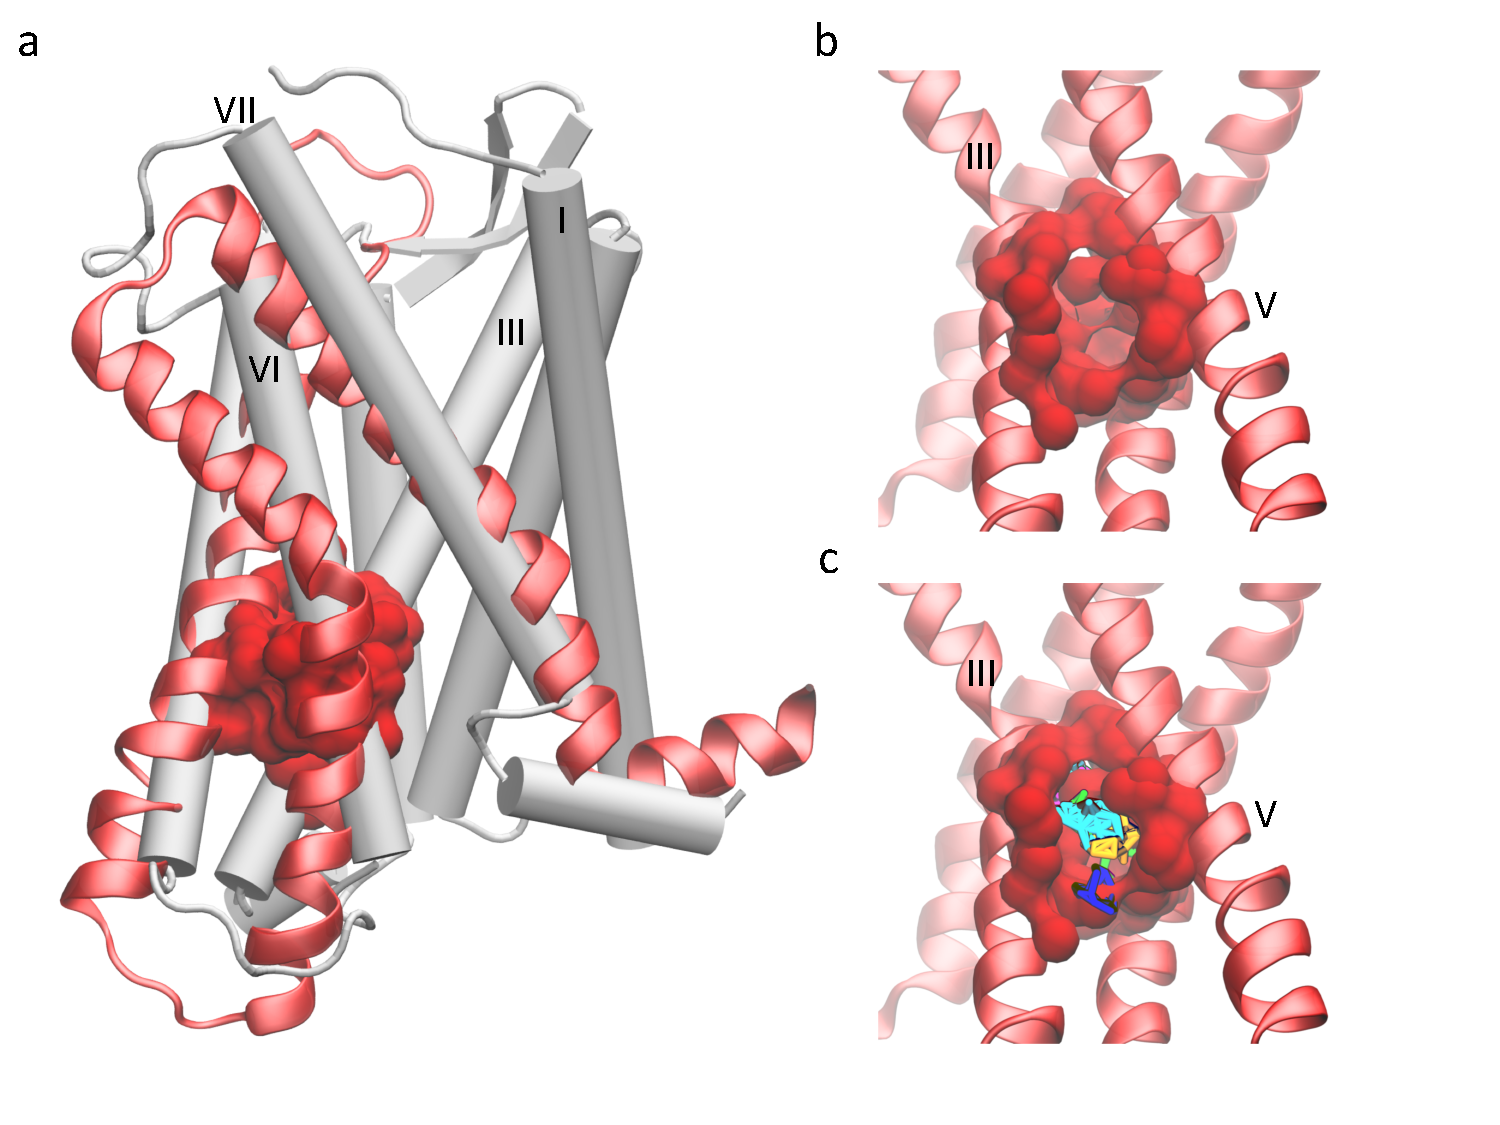
\includegraphics[width=8.6cm]{allo_pkt.pdf}
\caption{A putative allosteric drug binding pocket is revealed by three holo macrostates. A) A comparison of the CCR2 crystal structure (white cartoon) with helices V, VI, and VII (red new cartoon) of one holo macrostate. The pocket is shown in red surface. B) A closer view of the pocket from the other side of the protein, between helices III and V. C) Small organic probes used for computational fragment mapping are multicolored.}
\label{fig:allo_pkt}
\end{figure}

%%%% Discussion
\section*{Conclusions}

To characterize the basal dynamics of CCR2 and understand how small molecule antagonists modulate these dynamics, we coupled long timescale atomic simulations and MSM theory to compare the metastable states accessed by apo and holo CCR2 in its native membrane-embedded form. 
Antagonists perturb CCR2 dynamics and kinetics, and are associated with distinct residue rearrangement and key motions. 
Several intermediate states reveal a novel cryptic binding site that could be targeted with small molecule inhibitors. 
Without antagonists, CCR2 is able to access other distinct metastable states that are likely sampling along an activation pathway. These intermediate states inform on the basal dynamics of CCR2 and may be useful for modification of previously unsuccessful drugs.

%\subsection*{Digital Figures}
%Only TIFF, EPS, and high-resolution PDF for Mac or PC are allowed for figures that will appear in the main text, and images must be final size. Authors may submit U3D or PRC files for 3D images; these must be accompanied by 2D representations in TIFF, EPS, or high-resolution PDF format.  Color images must be in RGB (red, green, blue) mode. Include the font files for any text.


% \subsection*{Tables}
%In addition to including your tables within this manuscript file, PNAS requires that each table be uploaded to the submission separately as a “Table” file.  Please ensure that each table .tex file contains a preamble, the \verb|\begin{document}| command, and the \verb|\end{document}| command. This is necessary so that the submission system can convert each file to PDF.


%\subsection*{Supporting Information (SI)}

%Authors should submit SI as a single separate PDF file, combining all text, figures, tables, movie legends, and SI references.  PNAS will publish SI uncomposed, as the authors have provided it.  Additional details can be found here: \href{http://www.pnas.org/page/authors/journal-policies}{policy on SI}.  For SI formatting instructions click \href{https://www.pnascentral.org/cgi-bin/main.plex?form_type=display_auth_si_instructions}{here}.  The PNAS Overleaf SI template can be found \href{https://www.overleaf.com/latex/templates/pnas-template-for-supplementary-information/wqfsfqwyjtsd}{here}.  Refer to the SI Appendix in the manuscript at an appropriate point in the text. Number supporting figures and tables starting with S1, S2, etc.

\matmethods{
See the SI Appendix for full Materials and Methods.
MD trajectories and MSM construction scripts will be available for download.
\subsection*{\textbf{System Preparation and Molecular Dynamics Simulations}}
Two systems were simulated for a total of 260 $\mu$s: CCR2 holo, with both co-crystallized antagonist ligands bound, and CCR2 apo, without ligands bound. CCR2-RA-[R] and BMS 681\cite{Zheng2016} were deleted to build the apo system. Each all-atom system is embedded in a POPC bilayer, explicitly solvated with TIP3P, and simulated with 150mM NaCl, at pH 7.4, at 310K and 1 bar. The initial coordinates were taken from the experimental crystal structure\cite{Zheng2016}.

\subsection*{\textbf{Building the Markov State Models}}
TICA was used for dimensionality reduction and feature selection. 
The apo and holo systems were clustered separately using K-means. 
The MSMs were built with PyEMMA version 2.5.4 \cite{Scherer2015} and selected based on implied timescale plots (SI Appendix, Fig. S13) and Chapman-Kolmogorov tests (SI Appendix, Figs. S14,S15) and coarse-grained with hidden Markov models (HMMs).
Representative structures were selected from each macrostate by taking the centroid of the most populated microstate (SI Appendix, Figs. S16-S18)
}


\showmatmethods{}

\acknow{The authors thank Tracy Handel and Irina Kufareva for their valuable input as well as initial modification of CCR2 coordinates.
We thank Frank Noe and Cecilia Clementi for their useful discussions regarding MSM construction.
We also thank the organizers and participants of the 2018 Workshop on Free energy Methods, Kinetics and Markov State Models in Drug Design for helpful comments and discussion.
This work was supported in part by the Director's New Innovator Award Program NIH DP2-OD007237, the National Biomedical Computation Resource (NBCR) NIH P41-GM103426, and the National Science Foundation through XSEDE supercomputing resources provided via TG-CHE060073 to R.E.A.
C.T.L. also acknowledges support from the NIH Molecular Biophysics Training Program (T32-GM008326)
% This is block is copied directly from the PSC Anton 2 website.
Anton 2 computer time was provided by the Pittsburgh Supercomputing Center (PSC) through Grant R01GM116961 from the National Institutes of Health. The Anton 2 machine at PSC was generously made available by D.E. Shaw Research.
%%%%%
}
\showacknow{}

%\pnasbreak

% Bibliography
\bibliographystyle{plain}
\section*{References}
\bibliography{ccr2-0}
\end{document}